\documentclass[a4paper,twocolumn,8pt]{extarticle}

\usepackage[utf8]{inputenc}
\usepackage[english, russian]{babel}

\usepackage{extsizes}
\usepackage[a4paper,top=0.5cm,bottom=1.0cm,left=1.0cm,right=0.5cm,nomarginpar,foot=0.3cm,includehead]{geometry}
\usepackage{lastpage}
\usepackage{listings}
\usepackage{xcolor}
\usepackage{fancyhdr}
\usepackage{amssymb}
\usepackage{hyperref}
\usepackage{graphicx}

\hypersetup{
    colorlinks=true,
    linkcolor=black,
    filecolor=magenta,
    urlcolor=blue,
}

\definecolor{codegreen}{rgb}{0,0.6,0}
\definecolor{codegray}{rgb}{0.5,0.5,0.5}
\definecolor{codepurple}{rgb}{0.58,0,0.82}
\definecolor{backcolour}{rgb}{1,1,1}

\lstdefinestyle{codestyle}{
    language=C++,
    backgroundcolor=\color{backcolour},
    commentstyle=\color{codegreen},
    keywordstyle=\color{magenta},
    stringstyle=\color{codepurple},
    basicstyle=\ttfamily,
    breakatwhitespace=false,
    breaklines=true,
    captionpos=b,
    keepspaces=true,
    numbersep=5pt,
    showspaces=false,
    showstringspaces=false,
    showtabs=false,
    tabsize=2
}

\lstset{
    style=codestyle,
    extendedchars=\true,
%    literate=
%        {б}{{\selectfont\char225}}1
%        {в}{{\selectfont\char226}}1
%        {г}{{\selectfont\char227}}1
}
\setlength{\columnseprule}{0.4pt}
\setlength{\columnsep}{30pt}

\begin{document}
    \pagestyle{fancy}
    \fancyhead[LO]{St. Petersburg State University (Ushakov, Turevskii, Danilevich)}
    \fancyhead[R]{Page \thepage~of~\pageref{LastPage}}
    \tableofcontents
    \newpage
    \section{Теория чисел}
    \subsection{КТО}
\begin{lstlisting}
int gcd(int a, int b, int &x, int &y) {
  if (b==0) { x = 1; y = 0; return a; }
  int d = gcd(b,a%b,y,x);
  y-=a/b*x;
  return d;
}
int inv(int r, int m) {
  int x, y;
  gcd(r,m,x,y);
  return (x+m)%m;
}
int crt(int r, int n, int c, int m) { return r + ((c - r) % m + m) * inv(n, m) % m * n; }
\end{lstlisting}
% https://codeforces.com/contest/982/submission/230056019

    \subsection{Алгоритм Миллера --- Рабина}
\lstinputlisting{algos/miller rabin/miller rabin.cpp}
    \subsection{Алгоритм Берлекэмпа --- Месси}
\underline{\url{https://mzhang2021.github.io/cp-blog/berlekamp-massey/}}
\begin{lstlisting}
template<typename T>
vector<T> berlekampMassey(const vector<T> &s) {
  int n = (int) s.size(), l = 0, m = 1;
  vector<T> b(n), c(n);
  T ld = b[0] = c[0] = 1;
  for (int i=0; i<n; i++, m++) {
    T d = s[i];
    for (int j=1; j<=l; j++)
      d += c[j] * s[i-j];
    if (d == 0)
      continue;
    vector<T> temp = c;
    T coef = d / ld;
    for (int j=m; j<n; j++)
      c[j] -= coef * b[j-m];
    if (2 * l <= i) {
      l = i + 1 - l;
      b = temp;
      ld = d;
      m = 0;
    }
  }
  c.resize(l + 1);
  c.erase(c.begin());
  for (T &x : c)
    x = -x;
  return c;
}  
\end{lstlisting}

    \section{Графы}
    \subsection{$\mathcal{SCC}$ и 2-$\mathcal{SAT}$}
Алгоритм ищет сильносвязные компоненты в графе $g$, если есть путь $i \rightarrow j$, то $scc[i] \le scc[j]$

В случае 2-$\mathcal{SAT}$ рёбра $i \Rightarrow j$ и $(j\oplus1) \Rightarrow (i \oplus 1)$ должны быть добавлены одновременно.
\begin{lstlisting}
vector<vector<int>> g(2 * n);
vector<vector<int>> r(g.size());
for (int i = 0; i < g.size(); ++i) {
  for (int j : g[i]) r[j].push_back(i);
}
vector<int> used(g.size()), tout(g.size());
int time = 0;
auto dfs = [&](auto dfs, int cur) -> void {
  if (used[cur]) return;
  used[cur] = 1;
  for (int nxt : g[cur]) {
    dfs(dfs, nxt);
  }
  // used[cur] = 2;
  tout[cur] = time++;
};
for (int i = 0; i < g.size(); ++i) if (!used[i]) dfs(dfs, i);
vector<int> ind(g.size());
iota(ind.begin(), ind.end(), 0);
sort(all(ind), [&](int i, int j){return tout[i] > tout[j];});
vector<int> scc(g.size(), -1);
auto go = [&](auto go, int cur, int color) -> void {
  if (scc[cur] != -1) return;
  scc[cur] = color;
  for (int nxt : r[cur]) {
    go(go, nxt, color);
  }
};
int color = 0;
for (int i : ind) {
  if (scc[i] == -1) go(go, i, color++);
}
for (int i = 0; i < g.size() / 2; ++i) {
  if (scc[2 * i] == scc[2 * i + 1]) "IMPOSSIBLE"
  if (scc[2 * i] < scc[2 * i + 1]) {
    // !i => i, assign i = true
  } else {
    // i => !i, assign i = false
  }
}
\end{lstlisting}

%https://codeforces.com/contest/228/submission/230077013
%https://judge.yosupo.jp/submission/168750
%https://judge.yosupo.jp/submission/168753
    \subsection{Эйлеров цикл}
\begin{lstlisting}
vector<vector<pair<int, int>>> g(n); // pair{nxt, idx}
vector<pair<int, int>> e(p.size());
// build graph
vector<int> in(n), out(n);
for (auto [u, v] : e) in[v]++, out[u]++;
vector<int> used(m), it(n), cycle;
auto dfs = [&](auto dfs, int cur) -> void {
    while (true) {
        while (it[cur] < g[cur].size() && used[g[cur][it[cur]].second]) it[cur]++;
        if (it[cur] == g[cur].size()) return;
        auto [nxt, idx] = g[cur][it[cur]];
        used[idx] = true;
        dfs(dfs, nxt);
        cycle.push_back(idx);
    }
};
int cnt = 0, odd = -1;
for (int i = 0; i < n; ++i){
    if (out[i] && odd == -1) odd = i;
    if (in[i] != out[i]) {
        if (in[i] + 1 == out[i]) odd = i;
        if (abs(in[i] - out[i]) > 1) return {}; // must hold
        cnt++;
    }
}
if (cnt != 0 && cnt != 2) return {}; // must hold
// for undirected find odd vertex (and count that # of odd is 0 or 2)
dfs(dfs, odd);
reverse(cycle.begin(), cycle.end());
if (cycle.size() != m) return {};
\end{lstlisting}
% https://codeforces.com/gym/102935/submission/230083828
    \subsection{Компоненты рёберной двусвязности}
\begin{lstlisting}
int n, m;
cin >> n >> m;
vector <vector <int> > g(n + 1);
map <pair <int, int>, int> comp, col;
for (int i = 0; i < m; ++i) {
  int u, v, c; cin >> u >> v >> c;c--;
  col[{u,v}]=col[{v,u}]=c;
  g[u].push_back(v);
  g[v].push_back(u);
}
vector <int> used(n + 1);
vector <int> newCompWithoutParent(n + 1), h(n + 1), up(n + 1);
function <void(int,int)> findCutPoints = [&] (int u, int p) {
  used[u] = 1;
  up[u] = h[u];
  for (int v : g[u]) {
    if (!used[v]) {
      h[v] = h[u] + 1;
      findCutPoints(v, u);
      up[u] = min(up[u], up[v]);
      if (up[v] >= h[u]) {
        newCompWithoutParent[v] = 1;
      }
    }
    else {
      up[u] = min(up[u], h[v]);
    }
  }
};
for (int u = 1; u <= n; ++u) {
  if (!used[u]) {
    findCutPoints(u, u);
  }
}
int ptr = 0;
vector <map <int, int> > colors(m);
function <void(int, int)> markComponents = [&] (int u, int cur) {
  used[u] = 1;
  for (int v : g[u]) {
    if (!used[v]) {
      if (newCompWithoutParent[v]) {
        ptr++;
        markComponents(v, ptr - 1);
      }
      else {
        markComponents(v, cur);
      }
    }
    else if (h[v] < h[u]) {
      comp[{u,v}]=comp[{v,u}]=cur;
      int c = col[{u,v}];
      colors[cur][u] |= 1 << c;
      colors[cur][v] |= 1 << c;
    }
  }
};
used.assign(n + 1, 0);
for (int u = 1; u <= n; ++u) {
  if (!used[u]) {
    markComponents(u, -1);
  }
}
for (int comp = 0; comp < m; ++comp) {
  vector <int> cnt(4);
  int tot = 0;
  for (auto [u, mask] : colors[comp]) {
    tot |= mask;
    cnt[bp(mask)]++;
  }
  if (bp(tot)<3) {
    continue;
  }
  if (cnt[2] || cnt[3]>2) {
    cout << "Yes" << endl;
    return;
  }
}
cout << "No" << endl;  
\end{lstlisting}
% https://qoj.ac/submission/281898

    \section{\texttt{xor}, \texttt{and}, \texttt{or}-свёртки}
    \lstinputlisting{convolutions/convolutions.cpp}

    \section{Структуры данных}
    \subsection{Дерево Фенвика}
\begin{lstlisting}
int fe[maxn]; /// fenwick tree
void pl(int pos,int val) {while(pos<maxn) {fe[pos]+=val;pos|=(pos+1);}}
int get(int pos) {int ans=0;while(pos>=0) {ans+=fe[pos];pos&=(pos+1);--pos;} return ans;} /// [0,pos] - vkluchitelno!!!
int get(int l,int r) {return get(r-1)-get(l-1);} /// summa na [l,r)
\end{lstlisting}
    \subsection{Дерево отрезков}
\begin{lstlisting}
template<typename Data, typename Mod, typename UniteData, typename UniteMod, typename Apply>
struct MassSegmentTree {
  int h, n;
  Data zd;
  Mod zm;
  vector<Data> data;
  vector<Mod> mod;

  UniteData ud; // Data (Data, Data)
  UniteMod um; // Mod (Mod, Mod);
  Apply a; // Data (Data, Mod, int); last argument is the length of current segment (could be used for range += and sum counting, for instance)

  template<typename I>
  MassSegmentTree(int sz, Data zd, Mod zm, UniteData ud, UniteMod um, Apply a, I init) : h(__lg(sz > 1 ? sz - 1 : 1) + 1), n(1 << h), zm(zm), zd(zd), data(2 * n, zd), mod(n, zm), ud(ud), um(um), a(a) {
    for (int i = 0; i < sz; ++i) data[i + n] = init(i);
    for (int i = n - 1; i > 0; --i) data[i] = ud(data[2 * i], data[2 * i + 1]);
  }

  MassSegmentTree(int sz, Data zd, Mod zm, UniteData ud, UniteMod um, Apply a) : h(__lg(sz > 1 ? sz - 1 : 1) + 1), n(1 << h), zm(zm), zd(zd), data(2 * n, zd), mod(n, zm), ud(ud), um(um), a(a) {}

  void push(int i) {
    if (mod[i] == zm) return;
    apply(2 * i, mod[i]);
    apply(2 * i + 1, mod[i]);
    mod[i] = zm;
  }

  // is used only for apply
  int length(int i) { return 1 << (h - __lg(i)); }

  // is used only for descent
  int left(int i) {
    int lvl = __lg(i);
    return (i & ((1 << lvl) - 1)) * (1 << (h - lvl));
  }

  // is used only for descent
  int right(int i) {
    int lvl = __lg(i);
    return ((i & ((1 << lvl) - 1)) + 1) * (1 << (h - lvl));
  }

  template<typename S>
  void apply(int i, S x) {
    data[i] = a(data[i], x, length(i));
    if (i < n) mod[i] = um(mod[i], x);
  }

  void update(int i) {
    if (mod[i] != zm) return;
    data[i] = ud(data[2 * i], data[2 * i + 1]);
  }

  template<typename S>
  void update(int l, int r, S x) { // [l; r)
    l += n, r += n;
    for (int shift = h; shift > 0; --shift) {
      push(l >> shift);
      push((r - 1) >> shift);
    }
    for (int lf = l, rg = r; lf < rg; lf /= 2, rg /= 2) {
      if (lf & 1) apply(lf++, x);
      if (rg & 1) apply(--rg, x);
    }
    for (int shift = 1; shift <= h; ++shift) {
      update(l >> shift);
      update((r - 1) >> shift);
    }
  }

  Data get(int l, int r) { // [l; r)
    l += n, r += n;
    for (int shift = h; shift > 0; --shift) {
      push(l >> shift);
      push((r - 1) >> shift);
    }
    Data leftRes = zd, rightRes = zd;
    for (; l < r; l /= 2, r /= 2) {
      if (l & 1) leftRes = ud(leftRes, data[l++]);
      if (r & 1) rightRes = ud(data[--r], rightRes);
    }
    return ud(leftRes, rightRes);
  }

  // l \in [0; n) && ok(get(l, l), l);
  // returns last r: ok(get(l, r), r)
  template<typename C>
  int lastTrue(int l, C ok) {
    l += n;
    for (int shift = h; shift > 0; --shift) push(l >> shift);
    Data cur = zd;
    do {
      l >>= __builtin_ctz(l);
      Data with1;
      with1 = ud(cur, data[l]);
      if (ok(with1, right(l))) {
        cur = with1;
        ++l;
      } else {
        while (l < n) {
          push(l);
          Data with2;
          with2 = ud(cur, data[2 * l]);
          if (ok(with2, right(2 * l))) {
            cur = with2;
            l = 2 * l + 1;
          } else {
            l = 2 * l;
          }
        }
        return l - n;
      }
    } while (l & (l - 1));
    return n;
  }

  // r \in [0; n) && ok(get(r, r), r);
  // returns first l: ok(get(l, r), l)
  template<typename C>
  int firstTrue(int r, C ok) {
    r += n;
    for (int shift = h; shift > 0; --shift) push((r - 1) >> shift);
    Data cur = zd;
    while (r & (r - 1)) {
      r >>= __builtin_ctz(r);
      Data with1;
      with1 = ud(data[--r], cur);
      if (ok(with1, left(r))) {
        cur = with1;
      } else {
        while (r < n) {
          push(r);
          Data with2;
          with2 = ud(data[2 * r + 1], cur);
          if (ok(with2, right(2 * r))) {
            cur = with2;
            r = 2 * r;
          } else {
            r = 2 * r + 1;
          }
        }
        return r - n + 1;
      }
    }
    return 0;
  }
};
\end{lstlisting}
\subsubsection{Примеры использования}
\begin{itemize}
  \item Взятие максимума и прибавление константы
\begin{lstlisting}
MassSegmentTree segtree(n, 0LL, 0LL,
[](int x, int y) { return max(x, y); },
[](int x, int y) { return x + y; },
[](int x, int y, int len) { return x + y; });
\end{lstlisting}

  \item Взятие суммы и прибавление константы
\begin{lstlisting}
MassSegmentTree segtree(n, 0LL, 0LL,
[](int x, int y) { return x + y; },
[](int x, int y) { return x + y; },
[](int x, int y, int len) { return x + y * len; });
\end{lstlisting}

\item Взятие суммы и присовение
\begin{lstlisting}
MassSegmentTree segtree(n, 0LL, -1LL,
[](int x, int y) { return x + y; },
[](int x, int y) { return y; },
[](int x, int y, int len) { return y * len; });
\end{lstlisting}
\end{itemize}
    \subsection{Ordered set}
\lstinputlisting{algos/ordered set/ordered set.cpp}
    \subsection{Convex hull trick}
    \lstinputlisting{cht.cpp}
    \subsection{Центроидная декомпозиция}
    \lstinputlisting{centroids.cpp}

    \section{Строковые алгоритмы}
    \subsection{Префикс-функция}
\begin{lstlisting}
vector<int> prefix_function(string s) {
  vector<int> p(s.size());
  for (int i = 1; i < s.size(); ++i) {
    p[i] = p[i - 1];
    while (p[i] && s[p[i]] != s[i]) p[i] = p[p[i] - 1];
    p[i] += s[i] == s[p[i]];
  }
  return p;
}
\end{lstlisting}

    \subsection{Z-функция}
\begin{lstlisting}
vector<int> z_function (string s) { // z[i] - lcp of s and s[i:]
 int n = (int) s.length();
 vector<int> z (n);
 for (int i=1, l=0, r=0; i<n; ++i) {
  if (i <= r)
   z[i] = min (r-i+1, z[i-l]);
  while (i+z[i] < n && s[z[i]] == s[i+z[i]])
   ++z[i];
  if (i+z[i]-1 > r)
   l = i,  r = i+z[i]-1;
 }
 return z;
}
\end{lstlisting}
    \subsection{Алгоритм Манакера}
\begin{lstlisting}
vector<int> manacher_odd(const string &s) {
    vector<int> man(s.size(), 0);
    int l = 0, r = 0;
    int n = s.size();
    for (int i = 1; i < n; i++) {
        if (i <= r) {
            man[i] = min(r - i, man[l + r - i]);
        }
        while (i + man[i] + 1 < n && i - man[i] - 1 >= 0 && s[i + man[i] + 1] == s[i - man[i] - 1]) {
            man[i]++;
        }
        if (i + man[i] > r) {
            l = i - man[i];
            r = i + man[i];
        }
    }
    return man;
}
// abacaba : (0 1 0 3 0 1 0)
// abbaa : (0 0 0 0 0)

vector <int> manacher_even(const string &s) {
    assert(s.size());
    string t;
    for (int i = 0; i + 1 < s.size(); ++i) {
        t += s[i];
        t += '#';
    }
    t += s.back();
    auto odd = manacher_odd(t);
    vector <int> ans;
    for (int i = 1; i < odd.size(); i += 2) {
        ans.push_back((odd[i]+1)/2);
    }
    return ans;
}
// abacaba : (0 0 0 0 0 0)
// abbaa : (0 2 0 1)
\end{lstlisting}
    \subsection{Суфмассив}
Китайский суффмассив
\begin{lstlisting}
struct SuffixArray {
    vector <int> sa, lcp;
    SuffixArray (string &s, int lim=256) {
        int n = (int)s.size() + 1, k = 0, a, b;
        vector <int> x(s.begin(), s.end() + 1), y(n), ws(max(n, lim)), rank(n);
        sa = lcp = y, iota(sa.begin(), sa.end(), 0);
        for (int j = 0, p = 0; p < n; j = max(1ll, j * 2), lim = p) {
            p = j, iota(y.begin(), y.end(), n - j);
            for (int i = 0; i < n; i++) if (sa[i] >= j) y[p++] = sa[i] - j;
            fill(ws.begin(), ws.end(), 0);
            for (int i = 0; i < n; i++) ws[x[i]]++;
            for (int i = 1; i < lim; i++) ws[i] += ws[i - 1];
            for (int i = n; i--; ) sa[--ws[x[y[i]]]] = y[i];
            swap(x, y), p = 1, x[sa[0]] = 0;
            for (int i = 1; i < n; i++) a = sa[i - 1], b = sa[i], x[b] = (y[a] == y[b] && y[a + j] == y[b + j]) ? p - 1 : p++;
        }
        for (int i = 1; i < n; i++) rank[sa[i]] = i;
        for (int i = 0, j; i < n - 1; lcp[rank[i++]]=k)
        for (k && k--, j = sa[rank[i] - 1];
        s[i + k] == s[j + k]; k++);
    }
};
struct Rmq {
    const int INF = 1e9;
    vi rmq;
    int sz;
    Rmq(){}
    void build(int n) {
        sz = 1;
        while (sz < n) sz *= 2;
        rmq.assign(sz * 2, INF);
    }
    Rmq(int n) {
        sz = 1;
        while (sz < n) sz *= 2;
        rmq.assign(sz * 2, INF);
    }
    void put(int i, int x) {
        i += sz;
        ckmin(rmq[i], x);
        for (i/= 2; i; i/= 2) {
            rmq[i] = min(rmq[i * 2], rmq[i * 2 + 1]);
        }
    }
    int getMin(int l, int r) { //[l;r)
    assert(l < r);
    r--;
    l += sz;
    r += sz;
    int res = INF;
    while(l < r) {
        if (l%2 == 1) res = min(res, rmq[l]);
        if (r%2 == 0) res = min(res, rmq[r]);
        l = (l + 1)/2;
        r = (r - 1) /2;
    }
    if (l == r) res = min(res, rmq[l]);
    return res;
    }
};

struct Lc {
    vi pos;
    Rmq rmq;
    void build(string s) {
        SuffixArray sa(s);
        auto ss = sa.sa;
        ss.erase(ss.begin());

        auto lcp = sa.lcp;
        lcp.erase(lcp.begin());
        lcp.erase(lcp.begin());

        pos.resize(s.size());
        assert(s.size() == ss.size());
        FOR (i, ss.size()) {
            pos[ss[i]] = i;
        }
        int n = s.size();
        assert(lcp.size() == n - 1);
        rmq.build(n - 1);
        FOR (i, n - 1) {
            rmq.put(i, lcp[i]);
        }
    }
    int getLcp(int i, int j) {
        i = pos[i]; j = pos[j];
        if (j < i) {
            swap(i, j);
        }
        if (i == j) {
            return 1e18;
        }
        else {
            return rmq.getMin(i, j);
        }
    }
};
\end{lstlisting}

    \subsection{Алгоритм Ахо --- Корасик}
    \lstinputlisting{aho-corasick.cpp}
    \subsection{Дерево палиндромов}
    \lstinputlisting{palindromic.cpp}

    \section{Потоки}
    \subsection{Алгоритм Диница}
\begin{lstlisting}
#define pb push_back
struct Dinic{
struct edge{
    int to, flow, cap;
};

const static int N = 555; //count of vertices

vector<edge> e;
vector<int> g[N + 7];
int dp[N + 7];
int ptr[N + 7];

void clear(){
    for (int i = 0; i < N + 7; i++) g[i].clear();
    e.clear();
}

void addEdge(int a, int b, int cap){
    g[a].pb(e.size());
    e.pb({b, 0, cap});
    g[b].pb(e.size());
    e.pb({a, 0, 0});
}

int minFlow, start, finish;

bool bfs(){
    for (int i = 0; i < N; i++) dp[i] = -1;
    dp[start] = 0;
    vector<int> st;
    int uk = 0;
    st.pb(start);
    while(uk < st.size()){
        int v = st[uk++];
        for (int to : g[v]){
            auto ed = e[to];
            if (ed.cap - ed.flow >= minFlow && dp[ed.to] == -1){
                dp[ed.to] = dp[v] + 1;
                st.pb(ed.to);
            }
        }
    }
    return dp[finish] != -1;
}

int dfs(int v, int flow){
    if (v == finish) return flow;
    for (; ptr[v] < g[v].size(); ptr[v]++){
        int to = g[v][ptr[v]];
        edge ed = e[to];
        if (ed.cap - ed.flow >= minFlow && dp[ed.to] == dp[v] + 1){
            int add = dfs(ed.to, min(flow, ed.cap - ed.flow));
            if (add){
                e[to].flow += add;
                e[to ^ 1].flow -= add;
                return add;
            }
        }
    }
    return 0;
}

int dinic(int start, int finish){
    Dinic::start = start;
    Dinic::finish = finish;
    int flow = 0;
    for (minFlow = (1 << 30); minFlow; minFlow >>= 1){
        while(bfs()){
            for (int i = 0; i < N; i++) ptr[i] = 0;
            while(int now = dfs(start, (int)2e9 + 7)) flow += now;
        }
    }
    return flow;
}
} dinic;
\end{lstlisting}
    \subsection{Mincost k-flow}
\subsubsection{Строим граф}
\begin{lstlisting}
struct edge {
  int next, capacity, cost, flow = 0;

  edge() = default;

  edge(int next, int capacity, int cost) : next(next), capacity(capacity), cost(cost) {}

  int rem() const { return capacity - flow; }

  int operator+=(int f) { return flow += f; }

  int operator-=(int f) { return flow -= f; }
};
auto addEdge = [&](auto from, auto next, auto capacity, int cost) {
  g[from].push_back(e.size());
  e.emplace_back(next, capacity, cost);
  g[next].push_back(e.size());
  e.emplace_back(from, 0, -cost);
};
\end{lstlisting}
Если граф ориентированный, то addEdge вызываем один раз.
Если неориентированный, то два, вот так:
\begin{lstlisting}
addEdge(u, v, capacity, cost);
addEdge(v, u, capacity, cost);
\end{lstlisting}
\subsubsection{Запускаем Форда --- Беллмана}
\begin{lstlisting}
vector<ll> phi(n, 0);
auto fordBellman = [&](int s, int t) {
  phi.assign(n, 0);
  for (int iter = 0; iter < n; ++iter) {
    bool changed = false;
    for (int u = 0; u < n; ++u) {
      for (auto index : g[u]) {
        auto edge = e[index];
        if (edge.rem() > 0 && phi[edge.next] > phi[u] + edge.cost) {
          phi[edge.next] = phi[u] + edge.cost;
          changed = true;
        }
      }
    }
    if (!changed) break;
  }
};
fordBellman(s, t);
\end{lstlisting}

\subsubsection{Ищем кратчайший путь Дейкстрой с потенциалами}
\begin{lstlisting}
vector<ll> dist;
vector<int> from;
vector<bool> cnt;
auto dijkstra = [&](int s, int t) {
  dist.assign(n, 1e18);
  from.assign(n, -1);
  cnt.assign(n, false);
  dist[s] = 0;
  for (int i = 1; i < n; ++i) {
    int cur = find(cnt.begin(), cnt.end(), false) - cnt.begin();
    for (int j = 0; j < n; ++j) {
      if (!cnt[j] && dist[j] < dist[cur]) cur = j;
    }
    cnt[cur] = true;
    for (int index : g[cur]) {
      auto &edge = e[index];
      if (edge.rem() == 0) continue;
      ll weight = edge.cost + phi[cur] - phi[edge.next];
      if (dist[edge.next] > dist[cur] + weight) {
        dist[edge.next] = dist[cur] + weight;
        from[edge.next] = cur;
      }
    }
  }
  if (dist[t] == (ll) 1e18) return -1LL;
  ll cost = 0;
  for (int p = t; p != s; p = from[p]) {
    for (auto index : g[from[p]]) {
      auto &edge = e[index];
      ll weight = edge.cost + phi[from[p]] - phi[edge.next];
      if (edge.rem() > 0 && edge.next == p && dist[edge.next] == dist[from[p]] + weight) {
        edge += 1;
        e[index ^ 1] -= 1;
        cost += edge.cost;
        break;
      }
    }
  }
  for (int i = 0; i < n; ++i) {
    phi[i] += dist[i];
  }
  return cost;
};
ll cost = 0;
for (int flow = 0; flow < k; ++flow) {
  ll a = dijkstra(s, t);
  if (a == -1) {
    cout << "-1\n";
    return;
  }
  cost += a;
}
\end{lstlisting}
\subsubsection{Восстанавливаем ответ}
\begin{lstlisting}
auto findPath = [&](int s, int t) {
  vector<int> ans;
  int cur = s;
  while (cur != t) {
    for (auto index : g[cur]) {
      auto &edge = e[index];
      if (edge.flow <= 0) continue;
      edge -= 1;
      e[index ^ 1] += 1;
      ans.push_back(index / 4);
// index / 4 because each edge has 4 copies
      cur = edge.next;
      break;
    }
  }
  return ans;
};
for (int flow = 0; flow < k; ++flow) {
  auto p = findPath(s, t);
  cout << p.size() << ' ';
  for (int x : p) cout << x + 1 << ' ';
  cout << '\n';
}
\end{lstlisting}

    \section{FFT \& co}
    \subsection{NTT \& co}
\begin{lstlisting}
typedef long long ll;
const int p=998244353;
int po(int a,int b) {if(b==0) return 1; if(b==1) return a; if(b%2==0) {int u=po(a,b/2);return (u*1LL*u)%p;} else {int u=po(a,b-1);return (a*1LL*u)%p;}}
int inv(int x) {return po(x,p-2);}
template<int M, int K, int G> struct Fft {
  // 1, 1/4, 1/8, 3/8, 1/16, 5/16, 3/16, 7/16, ...
  int g[1 << (K - 1)];
  Fft() : g() { //if tl constexpr...
    static_assert(K >= 2, "Fft: K >= 2 must hold");
    g[0] = 1;
    g[1 << (K - 2)] = G;
    for (int l = 1 << (K - 2); l >= 2; l >>= 1) {
      g[l >> 1] = (static_cast<long long>(g[l]) * g[l]) % M;
    }
    assert((static_cast<long long>(g[1]) * g[1]) % M == M - 1);
    for (int l = 2; l <= 1 << (K - 2); l <<= 1) {
      for (int i = 1; i < l; ++i) {
        g[l + i] = (static_cast<long long>(g[l]) * g[i]) % M;
      }
    }
  }
  void fft(vector<int> &x) const {
    const int n = x.size();
    assert(!(n & (n - 1)) && n <= 1 << K);
    for (int h = __builtin_ctz(n); h--; ) {
      const int l = 1 << h;
      for (int i = 0; i < n >> 1 >> h; ++i) {
        for (int j = i << 1 << h; j < ((i << 1) + 1) << h; ++j) {
          const int t = (static_cast<long long>(g[i]) * x[j | l]) % M;
          if ((x[j | l] = x[j] - t) < 0) x[j | l] += M;
          if ((x[j] += t) >= M) x[j] -= M;
        }
      }
    }
    for (int i = 0, j = 0; i < n; ++i) {
      if (i < j) std::swap(x[i], x[j]);
      for (int l = n; (l >>= 1) && !((j ^= l) & l); ) {}
    }
  }
  vector<int> convolution(const vector<int> &a, const vector<int> &b) const {
    if(a.empty() || b.empty()) return {};
    const int na = a.size(), nb = b.size();
    int n, invN = 1;
    for (n = 1; n < na + nb - 1; n <<= 1) invN = ((invN & 1) ? (invN + M) : invN) >> 1;
    vector<int> x(n, 0), y(n, 0);
    std::copy(a.begin(), a.end(), x.begin());
    std::copy(b.begin(), b.end(), y.begin());
    fft(x);
    fft(y);
    for (int i = 0; i < n; ++i) x[i] = (((static_cast<long long>(x[i]) * y[i]) % M) * invN) % M;
    std::reverse(x.begin() + 1, x.end());
    fft(x);
    x.resize(na + nb - 1);
    return x;
  }
};
Fft<998244353,23,31> muls;
vector<int> form(vector<int> v,int n)
{
  while(v.size()<n) v.push_back(0);
  while(v.size()>n) v.pop_back();
  return v;
}
vector<int> operator *(vector<int> v1,vector<int> v2)
{
  return muls.convolution(v1,v2);
}
vector<int> operator +(vector<int> v1,vector<int> v2)
{
  while(v2.size()<v1.size()) v2.push_back(0); while(v1.size()<v2.size()) v1.push_back(0);
  for(int i=0;i<v1.size();++i) {v1[i]+=v2[i];if(v1[i]>=p) v1[i]-=p; else if(v1[i]<0) v1[i]+=p;}
  return v1;
}
vector<int> operator -(vector<int> v1,vector<int> v2)
{
  int sz=max(v1.size(),v2.size());while(v1.size()<sz) v1.push_back(0); while(v2.size()<sz) v2.push_back(0);
  for(int i=0;i<sz;++i) {v1[i]-=v2[i];if(v1[i]<0) v1[i]+=p; else if(v1[i]>=p) v1[i]-=p;} return v1;
}
vector<int> trmi(vector<int> v)
{
  for(int i=1;i<v.size();i+=2) {if(v[i]>0) v[i]=p-v[i]; else v[i]=(-v[i]);}
  return v;
}
vector<int> deriv(vector<int> v)
{
  if(v.empty()) return{};
  vector<int> ans(v.size()-1);
  for(int i=1;i<v.size();++i) ans[i-1]=(v[i]*1LL*i)%p;
  return ans;
}
vector<int> integ(vector<int> v)
{
  vector<int> ans(v.size()+1);ans[0]=0;
  for(int i=1;i<v.size();++i) ans[i-1]=(v[i]*1LL*i)%p;
  return ans;
}
vector<int> mul(vector<vector<int> > v)
{
  if(v.size()==1) return v[0];
  vector<vector<int> > v1,v2;for(int i=0;i<v.size()/2;++i) v1.push_back(v[i]); for(int i=v.size()/2;i<v.size();++i) v2.push_back(v[i]);
  return muls.convolution(mul(v1),mul(v2));
}
vector<int> inv1(vector<int> v,int n)
{
  assert(v[0]!=0);
  int sz=1;v=form(v,n);vector<int> a={inv(v[0])};
  while(sz<n)
  {
    vector<int> vsz;for(int i=0;i<min(n,2*sz);++i) vsz.push_back(v[i]);
    vector<int> b=((vector<int>) {1})-muls.convolution(a,vsz);
    for(int i=0;i<sz;++i) assert(b[i]==0);
    b.erase(b.begin(),b.begin()+sz);
    vector<int> c=muls.convolution(b,a);
    for(int i=0;i<sz;++i) a.push_back(c[i]);
    sz*=2;
  }
  return form(a,n);
}
vector<int> inv(vector<int> v,int n)
{
  v=form(v,n);assert(v[0]!=0);if(v.size()==1) {return {inv(v[0])};} vector<int> v1=trmi(v);
  vector<int> a=v1*v;a=form(a,2*n);
  vector<int> b((n+1)/2);for(int i=0;i<b.size();++i) b[i]=a[2*i];
  vector<int> ans1=inv(b,b.size());vector<int> ans2(n);for(int i=0;i<n;++i) {if(i%2==0) ans2[i]=ans1[i/2]; else ans2[i]=0;}
  return form(v1*ans2,n);
}
vector<int> operator/(vector<int> a,vector<int> b)
{
  while(!a.empty() && a.back()==0) a.pop_back(); while(!b.empty() && b.back()==0) b.pop_back();
  int n=a.size();int m=b.size();if(n<m) return {};
  reverse(a.begin(),a.end());reverse(b.begin(),b.end());vector<int> ans=a*inv(b,n-m+1);while(ans.size()>n-m+1) ans.pop_back();
  reverse(ans.begin(),ans.end());while(!ans.empty() && ans.back()==0) ans.pop_back();return ans;
}
vector<int> operator%(vector<int> a,vector <int> b)
{
  vector<int> ans=a-b*(a/b);while(!ans.empty() && ans.back()==0) ans.pop_back(); return ans;
}
\end{lstlisting}
    \section{Геома}
    \subsection{Касательные}
    \lstinputlisting{stress/tangents.cpp}
    \subsection{Примитивы}
    \lstinputlisting{geomPrim.cpp}
    \subsection{Точка нестрого внутри выпуклости}
    \lstinputlisting{inPolygon.cpp}
    \section{Разное}
    \subsection{Нимы}
По умолчанию проигрывает тот, кто не может сделать ход.
\begin{enumerate}
\item Полоска $1\times n$. Надо ставить крестик в незанятую клетку, нельзя ставить в соседние.
\textbf{Решение:} динамика за $\mathcal{O}(n^2)$. Оказывается, начиная с $n = 52$ есть период длины $34$.
\item Полоска $1\times n$. Надо ставить крестик в незанятую клетку. Выигрывает тот, кто получит три крестика подряд. \textbf{Решение:} как в (1), только крестик банит слева и справа по две клетки.
\item Доска $3 \times n$, изначально стоят $n$ белых пешек в первом ряду, $n$ чёрных в последнем. Правила шахматные, но бить обязательно. \textbf{Решение: } совпадает с (1).
\item Ним, но ещё за ход разрешается вместо взятия камней разделить какую-то кучку на две. \textbf{Решение:} динамика за квадрат. Оказывается, $g[n] = n + s_n$, где $s_n = 1$ для $n \equiv 3 \pmod{4}$, $s_n = -1$ для $n \equiv 0 \pmod {4}$, $s_n = 0$ в остальных случаях (и, конечно, при $n = 0$).
\item Полоска $1 \times n$. Надо поставить крестик в незанятую клетку, или пару крестиков в соседние незанятые клетки. \textbf{Решение:} динамика за квадрат. Оказывается, начиная с некоторого места $(n = 60?)$ последовательность периодична с периодом $12$.
\item $n$ кучек камней. Надо разделить кучку размера $\ge 3$ на две неравные. \textbf{Решение:} динамика за квадрат. Период неизвестен человечеству.
\item $n$ кучек камней. Надо переместить ненулевое число камней из $i$-й кучки в $(i-1)$-ю (для $i > 1$). \textbf{Решение:} нимбер --- это $a_2 \oplus a_4 \oplus a_6 \oplus \dots$, так как это ним с увеличениями.
\item Полоска $1 \times n$, на ней $k$ фишек. Надо переместить любую фишку куда-то влево, не перепрыгивая и не вставая на другие фишки. \textbf{Решение:} сводимся к предыдущей задаче
\item Полоска $1 \times n$, в каждой клетке $o$ илм $x$. Надо поменять $o$ на $x$, после чего (разрешается|надо) флипнуть знак где-то слева. \textbf{Решение:} нимбер --- $\oplus$-сумма координат нулей (в $1$|в $0$)-индексации.
\item Полоска $1 \times n$, в ней стоят две фишки $I$ и $I\:I$. Игрок берёт свою фишку, и перемещает на ненулевое число клеток, не перепрыгивая и не вставая на фишку противника. \textbf{Решение:} нимбер --- число клеток между фишками.
\item Доска $2 \times n$. Надо поставить крестики в $3$ незанятые клетки вида триомино (связная по сторонам фигура из трёх клеток, не лежащих на одной прямой). \textbf{Решение:} динамика за квадрат --- фигуру площади $n$ всегда можно разбить на $k$ и $n-3-k$.
\item Ним-Баше: можно брать не более $k$ предметов. \textbf{Решение: } эквивалентно ниму с состояниями $a_i \pmod{(k+1)}$.
\item Ним Мура: можно брать сколько угодно из не более, чем $k$ кучек. \textbf{Решение:} проигрышная тогда и только тогда если взять все кучки, записанные в двоичной системе счисления, то в каждом бите сумма делится на $(k+1)$.
\item Ним в поддавки: \textbf{Решение:} нимбер --- $a_1 \oplus \ldots \oplus a_n \oplus [\text{все }a_i \le 1]$.
\end{enumerate}
\subsection{Компараторы}
\lstinputlisting{algos/comparators guide.cpp}
\subsection{Трюки от Сергея Копелиовича}
\subsubsection{Быстрый ввод}
\underline{\url{https://acm.math.spbu.ru/~sk1/algo/input-output}}
\lstinputlisting{algos/fast-input.cpp}
\lstinputlisting{algos/read_double.cpp}
\underline{\url{https://acm.math.spbu.ru/~sk1/algo/memory.cpp.html}}
\subsubsection{Быстрый аллокатор}
\lstinputlisting{algos/bump-alloc.cpp}
\subsection{Редукция Барретта}
\lstinputlisting{algos/barrett.cpp}
\subsection{Флаги компияции}
\texttt{-DLOCAL -Wall -Wextra -pedantic -Wshadow -Wformat=2 -Wfloat-equal -Wconversion -Wlogical-op -Wshift-overflow=2 -Wduplicated-cond -Wcast-qual -Wcast-align -D\_GLIBCXX\_DEBUG -D\_GLIBCXX\_DEBUG\_PEDANTIC -D\_FORTIFY\_SOURCE=2 -fsanitize=address -fsanitize=undefined -fno-sanitize-recover -fstack-protector -std=c++2a}
%\subsubsection{Сеточка в vim}
%\underline{\url{https://codeforces.com/blog/entry/122540}}
%\begin{lstlisting}
%i|<esc>25A   |<esc>
%o+<esc>25A---+<esc>
%Vky35Pdd
%\end{lstlisting}
\subsection{Что сделать на пробном туре}
\begin{itemize}
\item Послать клар
\item Распечатать что-то
\item Получить ML (stack \& heap)
\item Максимальный размер отправляемого файла?
\item Убедиться, что чекер регистронезависимый (yes/YES)
\item Позапускать Флойда --- Варшалла
\item Посмотреть, насколько быстр быстрый ввод
\item Перебить что-то, проверить хеш
\item Проверить санитайзеры
\end{itemize}
\subsection{Хеш файла без комментариев}
Хеш файла, игнорирующий переводы строк и комментарии:
\begin{lstlisting}
$ cpp -dD -P -fpreprocessed "$filename" | tr -d '[:space:]' | md5sum | cut -c-6
\end{lstlisting}
\begin{verbatim}__builtin_ia32_ldmxcsr(40896);\end{verbatim}
    ...
%    \clearpage
%    
\includegraphics{hexagonal.ps}
%    \clearpage
%    \includegraphics{triangle.ps}
%    \clearpage
\end{document}